% Approach: combining CMB and time delay distances. Blinding.

% Results. Internal consistency. Consistency with other probes.

% Combination with stellar kinematics, introduces additional
% distance dependency. Not correlated, and weaker dependence than Ddt
% (See discussion with SHS about Jee et al papers)

Early approaches to inferring cosmological parameters from time delay
lens observations focused on measuring the Hubble constant in a
Friedman-Robertson-Walker model with asserted (fixed) density
parameters.\footnote{The original investigation by \citet{Ref64}
involved the ``assumption that the linear distance--red-shift relation
is valid.''} With better data came the recognition that time delay
lenses were really probes of cosmological distance
\citep{Koo++03,Suy++10}, and the emphasis shifted to
inferring the set of cosmological parameters that are needed  to predict
the kinematics of the expansion of the Universe out to the redshift of
the source.

The amount of cosmological information in an individual lens
is still relatively small, and the parameter most strongly constrained
is  the Hubble constant, but as sample sizes increase we expect
ensembles of  lenses to support the inference of several cosmological
parameters (or combinations thereof).

In Figure~\ref{fig:current-constraints} we reproduce the current best
constraints on  cosmological parameters, from the two best-measured
systems, B1608$+$656 and RXJ1131 \citep{Suy++14}. When this figure was
made, the available precision from just these two lenses was about the
same as that from SDSS DR7 BAO \citep{PercivalEtal2010} and the
``Constitution'' set of Type Ia supernovae \citep{HickenEtal2009}.
When all three of the curvature density $\Ok$, Dark Energy
density $\ODE$ and equation of state
$\wDE$ parameters are allowed to vary, along with $H_0$, we see that the
time delay lenses provide similar constraints to BAO and complementary
constraints to the SNe: the time delays and
the BAO signal depend on angular diameter distances and $H_0$, while
the supernovae probe luminosity distances.

%%%%%%%%%%%%%%%%%%%%%%%%%%%%%%%%%
\begin{figure*}[!ht]
\centering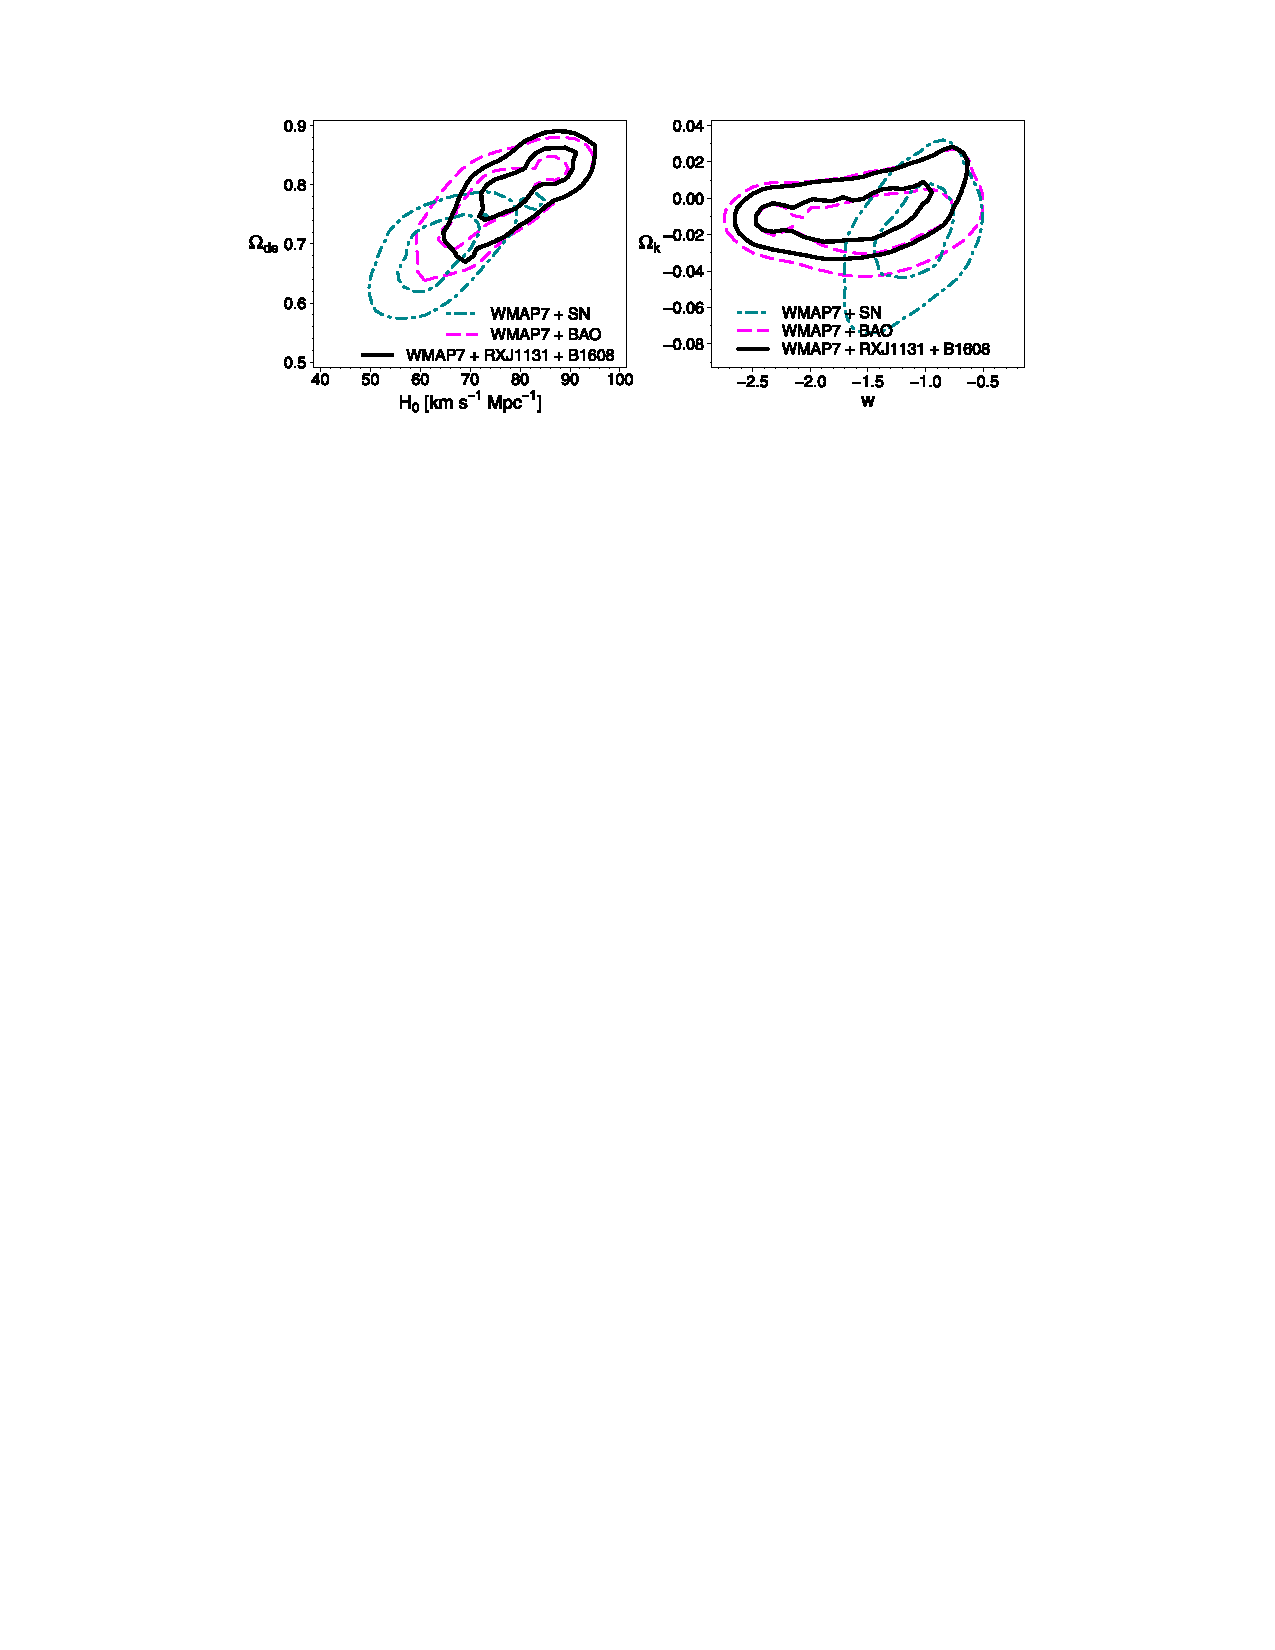
\includegraphics[width=0.9\linewidth]{figures/Suyu13_fig11.pdf}
\caption{Current cosmological parameter constraints from time delay
lenses. The marginalized posterior PDFs given the combined B1608$+$656
and RXJ1131 datasets and the assumption of an open CDM cosmology with
unknown dark energy equation of state is shown in
two sets of two parameter dimensions,
and compared to those given contemporary BAO and Type Ia supernova data.
Figure reproduced from \citet{Suy++14}.}
\label{fig:current-constraints}
\end{figure*}
%%%%%%%%%%%%%%%%%%%%%%%%%%%%%%%%%

One important feature of the cosmological parameter inference carried
out in the RXJ1131 analysis of \citet{Suy++13} is that it was blinded.
Following the simple methodology suggested in the blind Type Ia
supernova analysis of \citet{Con++06}, all cosmological parameter PDFs
were plotted with centroids offset to the origin until the team agreed
(after notably lengthy discussions about systematic errors) to ``open
the box.'' Such attempts to avoid ``unconscious experimenter bias''
introduced by stopping systematics analysis when the ``right answer'' is
obtained have long been advocated in particle physics
\citep{klein2005blind}, and seem likely to become the standard in
cosmology as well \citep[e.g.][]{STEP,DESWL}.

While the sample of very well-measured lenses was being painstakingly
expanded from zero to two, the exploration of statistical approaches to
dealing with large samples of lenses began.  Compressing the image
configuration and time delay in double image systems into a single
summary statistic, \citet{Ogu07b} derived a scaleable  method for
measuring the Hubble constant (but not the other cosmological
parameters) from samples of lenses, finding
$H_0=68\pm6\,{\rm(stat.)}\,\pm8\,{\rm (syst.)}\,{\rm km s}^{-1}{\rm
Mpc}^{-1}$ from a sample of 16 lenses with measured time delays. The
systematic uncertainties associated with this result may be hard to
reduce given the approximations made: while the summary statistic is
model-independent, the  interpretation is not. An alternative approach
is to work with more flexible lens models, fit the data for each one,
and combine the whole sample in a joint inference.  This is the approach
taken by \citet{Sah++06}, who found  $72^{8}_{11}\,{\rm km s}^{-1}{\rm
Mpc}^{-1}$ from 10 lenses (again assuming fixed curvature and dark energy
parameters). With the  non-parametric (pixelated) mass
models used, the degeneracy between  density profile slope and predicted
time delay is broken by the choice  of pixel value prior PDF. This assumption was
tested by \citet{Rea++07}, who used a hydrodynamic simulation of an
elliptical galaxy to generate mock image position and time delay data,
and confirm the accuracy of the previous study's Hubble constant
uncertainties. With improved time delay estimates in a sample
of ten lenses, \citet{RK++2015} reduced the uncertainty to
$\pm6\,{\rm km s}^{-1}{\rm Mpc}^{-1}$. While focused only on the
Hubble constant and carried out unblind, and with the lens environment and
line of sight mass structures remain unaccounted for and further tests
on realistic simulated galaxies warranted, these ensemble studies
point the way towards a future of considerably larger sample sizes.


Da as well as Ddt.
